\section{Endelige metode}
\subsection{Metoderne}
\subsubsection{Sparse Label Dictionaries}	% Marcus
%\textbf{Disclaimer der måske skal med: SLD er en metode udviklet af Anders noget fra DTU, vi har set metoden til et foredrag men har ikke set noget litteratur der beskriver metoden udførligt. Dette er derfor vores udlægning af SLD-metoden}\\
%\\
%SLD er en metode til at klassificere forskellige elementer i et givent billede. I SLD vælger man et passende udsnit af kandidatbilledet hvorefter 


%Sparse Label Dictionaries-metoden (SLD) vælger man et passende udsnit af kandidatbilledet således at udsnittet kommer til at indeholde de forskellige klasser af elementer man ønsker at dedektere samt

Sparse Label Dictionaries metoden (SLD) har til formål at segmentere billeder. SLD opretholder to matricer med information om image patches, den ene indeholder intensiteten og den anden den assosierede label information.

SLD opbygger disse to matricer i to trin, første trin er at initialisere matricen. Dette gøres ved at se på to billeder, et træningsbillede samt et billede hvor ground truth er markeret. Fra starten vælges så en størrelse på det udsnit man ønsker at arbejde med. En atom klippes så ud af træningsbilledet i pixel (0,0) og med størrelse $\sqrt{n}\times\sqrt{n}\times h$, hvor $n$ er antallet af pixels i udsnittet og h er farvedybten, så f.eks. 1 ved grayscale og 3 ved RGB billeder. Denne atom gemmes så i intensitetsmatricen. I præcis samme område klippes en atom ud af ground truth billedet der så gemmes i labelmatricen. En skematisk illustration af denne proces ses i figur \ref{fig:postmethod_intensitydict_init} og \ref{fig:postmethod_labeldict_init}. Ground truth billedet har også h dimensioner, hvor hvert segment der ønskes at detekteres er markeret men en farve. Vores udsnit flyttes så en pixel, hvorefter det samme gøres igen. Det vil sige at hvis træningsbilledet er $m\times m$ og vores atom størrelse er $n\times n$ så samler vi $(m-n+1)^2$ billeder. 

\begin{figure}[H]
		\centering
		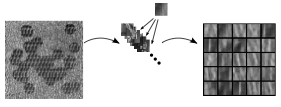
\includegraphics[scale=1]{files/postmethod/img/dict_1.png}
	\caption{Billedudsnit ekstraheret fra træningsbilledet og lagt over i intensitetsmatricen. \label{fig:postmethod_intensitydict_init}}
\end{figure}

\begin{figure}[H]
		\centering
		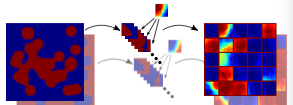
\includegraphics[scale=1]{files/postmethod/img/dict_2.png}
	\caption{Det tilsvarende ground truth billede med associerede udsnit ekstraheret og lagt i labelmatricen.\label{fig:postmethod_labeldict_init}}
\end{figure}

For at bygge de mest optimale billeder, ønsker vi at labelmatricen indeholder unikke billeder for hver klasse. Dette gøres ved at der vælges et tilfældigt subset af udsnittene fra træningsbilledet, og ved en iterativ proces, undersøges det hvorvidt det associerede labelatom allerede er tilnærmelsesvis repræsenteret i labelmatricen, og tilføjes kun hvis det ikke er tilfældet. Dette sikrer både at størrelsen på matricerne bliver minimeret der gør at listen er hurtigere at gennemgå, samt at billedudsnit med lignende intensiteter og labels tilhører samme matriceatomer. 

Når matricerne er fyldt op med intensitet- og labelatomer begynder en ny algoritme at optimere på matricernes indhold. Ideelt set vil en pixel i en labelatom have sandsynligheden 1 for en klasse og 0 for alle andre klasser. Algoritmen forsøger at opnå dette ved iterativt at opdele atomerne i klasser og redigere i label sandsynlighederne. 

Med de færdigbyggede matricer kan SLD gå igang med at segmentere billeder. Metoden starter typisk med at modtage et testbillede der bare kan være testbilledet med akserne ombyttet. Denne proces er dog kun for at teste at de matricer man har opbygget rent faktisk kan segmentere de klasser man ønsker.

\begin{figure}[H]
		\centering
		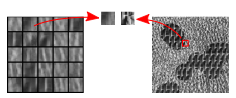
\includegraphics[scale=1]{files/postmethod/img/dict_3.png}
	\caption{\label{fig:postmethod_sld_imagepatch}}
\end{figure}

Processen med at segmentere et billede med de to matricer starter ligesom når matricerne blev opbygget. Udsnit størrelsen på $\sqrt{n}\times\sqrt{n}$ vælges, hvor $n$ igen er antallet af pixels i udsnittet, og løber igennem det billedet der ønskes segmenteret på samme vis som da vi fyldte matricerne. For hvert udsnit findes den atom, $d^*$, i intensitetsmatricen som Euklidisk ligger tættest på billedudsnittet ved ligningen
\begin{align}
	d^* = min_j ||d_j-x||
\end{align}

Dette er skematisk illustreret i figur \ref{fig:postmethod_sld_imagepatch}, hvor firkanten til højre repræsenterer det billede der ønskes segmenteret, og firkanten til venstre repræsenterer intensitetsmatricen. 

Herefter hentes den tilsvarende label ud fra labelmatricen og tilføjes til det nye segmenterede billede. Hver atom man tilføjer til det nye billede adderes oveni de allerede indsatte pixels hvilket betyder at hver pixel i det resulterende billede består af bidrag fra $n$ labelatom pixels, og som er et gennemsnit af sandsynlighederne af alle labels der dækker denne pixel. Denne labeling proces ses illustreret i figur \ref{fig:postmethod_sld_labelpatch}. Bemærk at siden dette er en binær segmentering, så har labelatomet to label dimensioner.  

Labelbilledet med den højeste intensitet bestemmer så det resulterende binære billede. Et eksempel på dette, hvor labelprocessen er halvejs ses i figur \ref{fig:postmethod_sld_resulting}.

\begin{figure}[H]
		\centering
		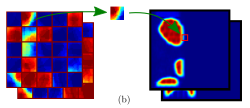
\includegraphics[scale=1]{files/postmethod/img/dict_4.png}
	\caption{\label{fig:postmethod_sld_labelpatch}}
\end{figure}

\begin{figure}[H]
		\centering
		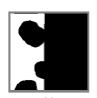
\includegraphics[scale=1]{files/postmethod/img/dict_5.png}
	\caption{\label{fig:postmethod_sld_resulting}}
\end{figure}

Skaberne af SLD beskriver metoden som værende en forbedring i forhold til andre lignende metoder, da den kun indeholder en matrice af intensitetsatomer selvom der er flere klasser. Samtidig er metoden stærk selv overfor billeder med meget støj og træningsbilleder med labels i dårlig kvalitet. I figur \ref{fig:postmethod_sld_testing} vises i første linje tre testbilleder med hhv. 5, 16, 10 og 2 klasser der skal segmenteres. I anden linje ses ground truth af disse billeder. I tredie linje ses resultatet efter segmenteringen. Her ses det tydeligt at hver klasse er segmenteret og der kun er segmenteringsfejl i overgangen mellem klasserne. Billederne er bl.a. behandlet med et gaussisk filter med standard afvigelse på 1.5 og udsnitstørrelse på $3\times3$.

\begin{figure}[H]
		\centering
		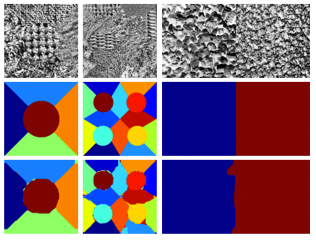
\includegraphics[scale=1]{files/postmethod/img/dict_6.png}
	\caption{\label{fig:postmethod_sld_testing}}
\end{figure}


\subsubsection{Foldning med eksempelbilleder} % Marcus
\subsubsection{Kombinationen} % Marcus
\subsection{Evaluering}
\subsubsection{ROC}
\subsubsection{Forbedringer af endelige metode}
\subsubsection{Hvad arbejder andre med} %
